\RequirePackage[l2tabu, orthodox]{nag}
\documentclass[a4paper]{article}
\usepackage[utf8]{inputenc}
\usepackage[T1]{fontenc}
\usepackage{bm}
\usepackage{caption}
\usepackage{listings}
\usepackage{booktabs}
\usepackage{mathtools}
\usepackage{algorithmic}
\usepackage{graphicx}
\usepackage{courier}
\usepackage{amsmath}
\usepackage{amssymb}
\usepackage{algorithm}
\usepackage[backend=biber]{biblatex}
\usepackage[font=small,labelfont=bf]{caption}

\DeclareMathOperator{\atantwo}{atan2}
\DeclarePairedDelimiter\floor{\lfloor}{\rfloor}

\addbibresource{report.bib}

\title{\textbf{Obstacle Avoidance} \\
	\textit{Deep Learning for Distance Estimation Using Optical or LIDAR Data}}
\author{\textbf{David Bergström} davbe125 \and \textbf{Martin Estgren} mares480 \and
\textbf{Sebastian Maghsoudi} sebma654 \and \textbf{Vincent Déhaye} vinde799}

\begin{document}
\maketitle
\newpage

\section{Introduction}

This project has examined two approaches to estimating distances from a given spatial position to objects in the environment. The two methods are LIDAR-based tracking and camera-based tracking.

\subsection{Background}
\subsection{Goals and Research Questions}

\subsubsection{LIDAR Tracking}

The aim of the paper is to replicate the result of the paper DeepTracking by Peter Ondruska and Ingmar Posner~\cite{DBLP:journals/corr/OndruskaP16}.

\subsubsection{Camera Tracking}

In this project we will examine if it is possible to use the SORT algorithm in order to track and estimate distances to people using a monocular camera system.  

\subsection{Content}

The reports is divided into two parts, one covering the LIDAR part of the project and one covering the camera tracking.
The sections method, result and discussion is divided into separate sections for the two project parts, while theory and conclusion sections are more mixed and covers both parts.

\subsubsection{LIDAR Tracking}

In the theory-section there will be a short summary of the paper introducing DeepTracking \cite{DBLP:journals/corr/OndruskaP16}.
Then, the method will be explained, outlining critical parts of training the network, preprocessing data and the overall architecture of the network.
After that, some details of the training of the network as well as an evaluation of the performance of the network.
Lastly, in the discussion part, the known and unknown differences between the implementations will be discussed

\subsubsection{Camera Tracking}

The theory section describe the two methods implemented, that is the detection and the tracking method.
The method will on an abstract level, describe how the goal and research question will be answered.
The implementation will then proceed to technically describe the realization of the method.
The discussion will put the method into real world perspective. And the conclusion will simply answer the research question.

\section{Theory}

\subsection{Detection}

Detection will here be defined as the process of detecting relevant objects and highlight them somehow for future processes, this is commonly done by assigning bounding boxes to the detected object. The detection is done frame by frame with different methods.
Since this paper reflects and revolves around the attempt to apply some algorithms to obstacle avoidance, it is perforce to define relevant obstacles.
In this case the focus is to avoid humans which gives the research an angle where there may be more simple to find already proven methods for the specific scenario.
Using different visual recognition application which was slightly modified to detect pedestrians, Dollár et al.~\cite{dollar2014fast} was able to display their efficiency in the relevant context.
An option to the, by Dollárs\cite{dollar2014fast} proposed, methods is convolutional neural network (CNN) based detectors.

\subsubsection{FrCNN}

% Be consistent with casing
FrCNN can a use a Region Proposal Network (RPN) that, given an image, generate so called object proposals \cite{NIPS2015_5638}.
With the object proposal, there is also a so called \textit{objectness} score.
This can then be inputed to FrCNN which then can be used to process through several convolutional layers in order to produce a feature map \cite{girshick2015fast}. 

\subsection{Tracking}

Tracking is here defined as the process of tracking detected objects frame to frame and assigning an identification to them.
% TODO: What happens here? The sentence just stops. Error in version control? Removed. I do not know waht was suppose the be there.

\subsubsection{SORT}

\emph{Simple Online and Real Tracking}, in this document abbreviated as SORT, is presented by Bewly et al.~\cite{Bewley2016_sort} as an combined approach of detecting and tracking objects in a video-feed.

The method was implemented to solve the problem of multiple object tracking, for example the type of tracking presented in the \emph{MOT challenge}\footnote{https://motchallenge.net/}.
SORT views the problem as association problem where the tracking is equivalent to associate the same detected objects in different frames.

\subsection{DeepTracking}

DeepTracking is an neural network architecture by Peter Ondruska and Ingmar Posner~\cite{DBLP:journals/corr/OndruskaP16}.
It provides end-to-end solution for tracking objects in data from a LIDAR.
End-to-end in this context meaning that the problem is solved using a neural network, taking preprocessed LIDAR data as input and outputting an occupancy grid.
Accompanying the paper is an implementation of the network, complete with training data \footnote{Available at \url{https://github.com/pondruska/DeepTracking}}.
The neural network has a hybrid architecture, combining recurrent neural networks and convolutional neural networks.

\section{Method}

\subsection{Camera Tracking}

A possible approach to using \emph{object tracking} for obstacle avoidance is to estimate the distances to each detected object. In this project, we divided the problem into three distinct parts.
\begin{figure}[H]
  \begin{center}
    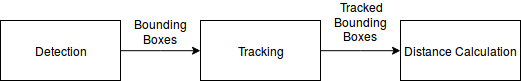
\includegraphics[width=1\textwidth]{figures/Moudule_diagram}
  \end{center}
  \caption{The abstract module diagram with the output/input for each module. }
  \label{fig:Mod_dia}
\end{figure}
Internally, the three parts work with \emph{bounding boxes} and the distances are only predicted in the final stage.

Figure \ref{fig:Mod_dia} does not take into account the input for the detection part (which would be a video frame) or output of the distance prediction (this would be a bounding box with corresponding distance).

\subsubsection{Detection}

The detection will as previously mentioned use a frame as input to apply the detection on.
The detection works in a couple of steps that produces bounding boxes that describes the coordinates for the upper-leftmost and lower-rightmost coordinate for each bounding box.
The first step is to generate so called object proposals that might be considered objects.
The object proposals are then considered when generating bounding boxes for each class/label e.g. person, aeroplane, car etc.
When generating the bounding boxes, a score is also appended that would correspond to the probability that the proposed object is of type class in question.
Assuming that a lower threshold for the score is applied, the proposed object of type class that does not pass the threshold is disregarded.

\begin{figure}[H]
  \begin{center}
    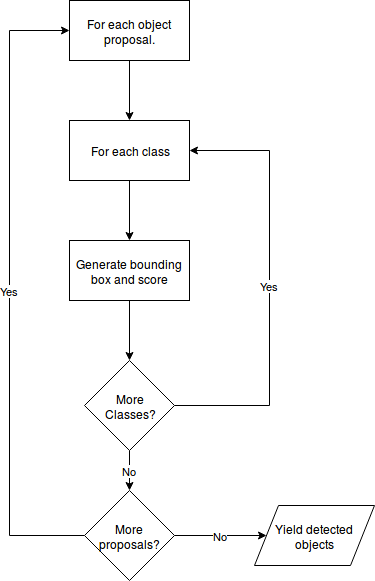
\includegraphics[width=0.8\textwidth]{figures/Detection_flow}
  \end{center}
  \caption{ Flow of the detection algorithm.}
  \label{fig:Det_flow}
\end{figure}

In figure \ref{fig:Det_flow} it becomes clear if we assume that given proposal and class that time complexity of generating bounding box is \(t=O(x)\) then the total complexity would be \(t_{tot}=O(x\alpha\beta)\) where \(\alpha\) correspond to the number of classes and \(\beta\) correspond to the object proposals.

\subsubsection{Tracking}

Tracking, in contrast to detection, only considers the bounding boxes them self.
Given a bounding box in one frame there are some parameters that can be used to consider if a bounding box in another frame correspond to the same object as in the first.
The most obvious parameter is the time between the frames, which is disregarded by assuming that the frames are consecutive frames from a video.

The second are the position of the bounding box.
In accordance with SORT\cite{Bewley2016_sort}, if a bounding box is not in a given amount of frames it is assumed not to exist in the frame any longer.

All this is as is previously mentioned to be considered as a association problem that in turn will be solved by a Kalman filter.

\subsubsection{Distance Calculation} \label{sec:DC}

Assuming the Pinhole camera model\cite{Sturm2014} one can continue to derive some additional information from the position of the bounding box.

If one first disregard the fact that the projection is inverted, one can derive some true proportions.
From the model one can assume \(\dfrac{x_{p}}{X_P}=\dfrac{y_{p}}{y_P}=\dfrac{f_{p}}{Z_P}\) where p is the projection point, the small coordinates (x and y) correspond to the projection and the large coordinates (X,Y and Z) correspond to the point in the scene and f is the focal length.

Given a standard height of an object and assuming that the difference to that height and the corresponding bounding box height is negligible one can use the same proportion to calculate the distance since that proportion would equal the proportion between Z and f.
Then yielded distance would be \(d=\sqrt{X^2+Y^2+Z^2}\). 


\subsection{LIDAR Tracking}

The method is based heavily on the method in paper DeepTracking by Peder Ondruska and Ingmar Posner~\cite{DBLP:journals/corr/OndruskaP16}.
The dataset, preprocessing steps, the network structure and loss function are the same as the paper.

The dataset is publicly available online \footnote{\url{http://mrg.robots.ox.ac.uk:8080/MRGData/deeptracking/DeepTracking_1_1.t7.zip}} and contains the LIDAR data from a sensor standing at a fixed location and a varying number of circular objects moving around it.
The objects all have the same size and move at a constant velocity, while the speed and the direction is random and varies from object to object.
In the file there is a large matrix with the dimensions $10000000 \times 721$.
Every row contains one sweep from the LIDAR sensor, the LIDAR sweeps fast from one angle to another recording the distance from the sensor to the first object the light hits at constant intervals.
Every row is processed into a 2-channel 2D occupancy grid with the dimensions $50 \times 50$.
The first channel of the grid describes the whether a grid cell contains an observation or not, while the second channel describes if a grid point is occluded or not.
The result of this preprocessing is a matrix with with the dimensions $10000000 \times 50 \times 50 \times 2$.

\subsubsection{Preprocessing of LIDAR Data}

Now, the preprocessing will be explained in more detail.
The sweep starts at a certain angle and records the distance from the sensor to the first object the light hits at constant intervals.
In the provided dataset the sweep starts at -180 degrees and does 721 recordings with the step size of 0.5 degrees.

First, the coordinate system is defined as top-down with the robot at the origin and the left being negative $x$ and in front of the robot is the negative $y$.

The matrix D is calculated, containing the Euclidean distance from the robot to a certain grid cell.
This is done by iterating over the grid and simply using the Pythagorean equation, resulting in a matrix:
\[
D_{i,j} = \sqrt{x_i^2 + y_j^2}
\]
The resulting matrix is visualized in figure \ref{fig:distance_matrix}.

\begin{figure}
  \begin{center}
    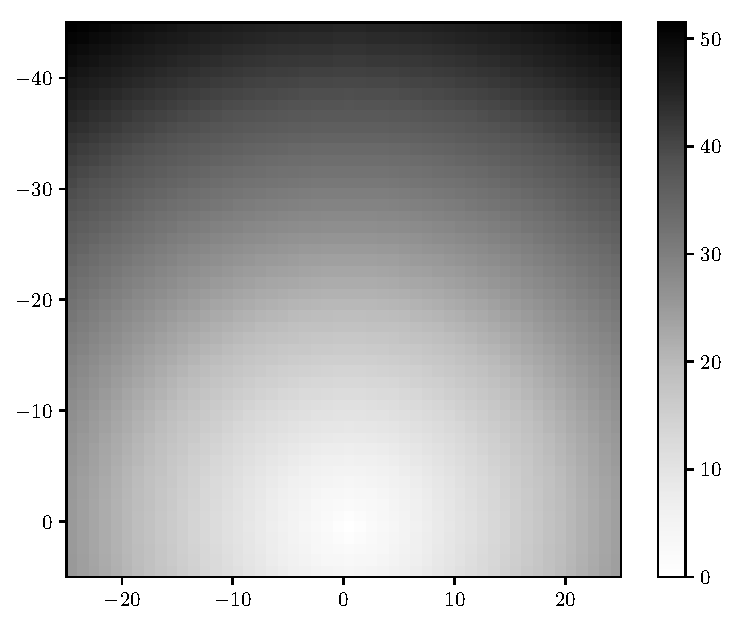
\includegraphics[width=0.5\textwidth]{figures/distance_matrix}
  \end{center}
  \caption{
    The distance matrix visualized, the robot exists at position $(0, 0)$.
    }
  \label{fig:distance_matrix}
\end{figure}

Then an index matrix is calculated, containing the index of LIDAR measurement corresponding to a certain grid cell.
Since the LIDAR measures in straight lines from the robot position, one measurement point will correspond to an entire line on the grid.
The angle between the robot and the grid cell is calculated, the angle is then used to calculate what index in the LIDAR vector the grid cell corresponds to.
More precisely, with the start angle $\alpha_0$ and step size $\delta$:
\[
I_{i, j} = \floor*{\frac{\atantwo(x_i, y_j) - \alpha_0}{\delta} + 0.5}
\]
The resulting matrix is visualized in figure \ref{fig:index_matrix}.

\begin{figure}
  \begin{center}
    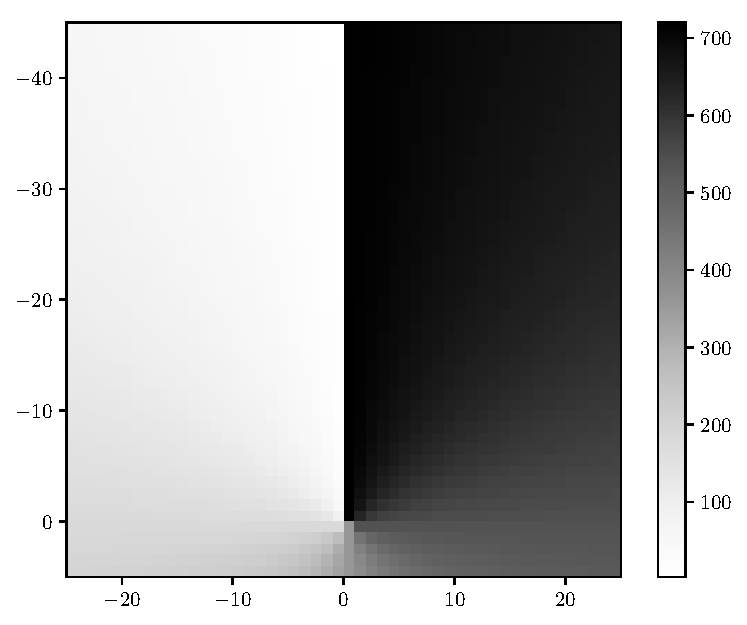
\includegraphics[width=0.5\textwidth]{figures/index_matrix}
  \end{center}
  \caption{
    The index matrix visualized, the robot exists at position $(0, 0)$.
    Note how index 0 is defined as straight ahead and how the index increases anti-clockwise, always going in straight lines from the robot's position.
    }
  \label{fig:index_matrix}
\end{figure}

Using these two matrices, it is then possible to calculate the wanted 2-channel image.
Note that the two matrices can be computed once for the entire time series.
The first channel of the output image represents whether a cell contains an observation or not.
This is calculated by taking the distance between the position the cell represents and the robot and then comparing it to the distance observed in the raw LIDAR data U.
Expressed in terms of the previously defined matrices:
\[
Y_{i, j, 1} = | U[I_{i, j}] - D_{i,j} | < \sqrt{2} \cdot \text{grid size}
\]
The second channel of the output image represents whether a cell is occluded by an observation or not.
\[
Y_{i, j, 2} = U[I_{i, j}] + \sqrt{2} \cdot \text{grid size} > D_{i, j}
\]
The two channels are visualized in figure \ref{fig:preprocessed_image}.

\begin{figure}
  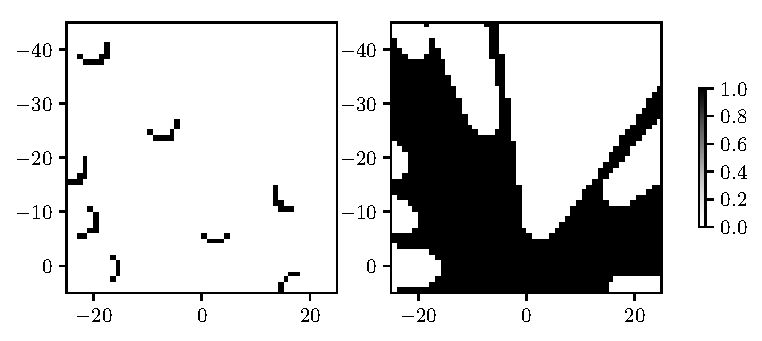
\includegraphics[width=\textwidth]{figures/preprocessed_image}
  \caption{
    LIDAR data sequence 721 preprocessed from using the method described.
    The left image is a channel 1 and the right image is channel 2.
    }
  \label{fig:preprocessed_image}
\end{figure}

\subsubsection{Network Structure}

The network structure is a combination of a recurrent neural network (RNN) and a convolutional neural network (CNN).
It combines the two types of architecture by having all layers be convolutional layers from CNNs while keeping the output from one of the layers between frames, making it also a RNN.
This allows it to keep information about objects in order to successfully track them between frames, even if the objects are temporarily occluded.

The networks consists of three convolutional layers, which are described by the original authors as: \emph{encoder}, \emph{belief tracker} and \emph{decoder}.
In the original paper, the kernel sizes and number of channels of output for the different layers were chosen.
These hyper parameters were not re-evaluated for this project.

All layers are convolutional layers with varying kernels size and number of output channels and the activation function sigmoid is applied element-wise to all outputs.
The convolutional layers use padding to keep the same dimensions of the image throughout the network ($50 \times 50$), but with a varying amount of channels.
The first layer is called the \emph{encoder} and has the kernel size $7 \times 7$ and 8 output channels.
Then, the output from the \emph{encoder} and the output of the \emph{belief tracker} from the previous iteration is concatenated, forming a 24 channel image.
The resulting 24 channel image is then fed into the second layer, which is called the \emph{belief tracker}.
The \emph{belief tracker} has the kernel size $5 \times 5$ and 16 channels of output.
The third and last layer has the name \emph{decoder} and takes the output of the \emph{belief tracker} as input, has a kernel size of $7 \times 7$ and outputs only one channel.

\subsubsection{Training the Network}

The network is trained in an unsupervised manner.
There are two major things the network should be able to do: predict movements of all objects and predict location of occluded objects.

In order to get the first property, some images of the input data to the network is left out.
More specifically the network is fed sequences of 100 images, but images 10-20, 30-40, 60-70, 90-100 are left out.
However, the loss function compares the full sequence of images with the predictions from the network.
This allows the network to be trained in an unsupervised manner and the network will learn to predict at least 10 time steps into the future.

% Describe loss-function
In order to get the second property, the loss function is masked in a way which does not give any loss to predictions in areas which are occluded by any objects.
Remember, the first channel of the input contains whether a grid cell contains an observation or not, while the second channel describes if a grid point is occluded or not.
The loss function uses the second channel as a mask, this means that no loss is given to a cell which is occluded.
The first channel is what is actually compared with the prediction from the network, using the cross-entropy loss function.
This means that the network is trained to predict the location observable objects, but is not given any penalty for predicting the position of non-observable objects.
This does not explicitly model the network to model objects which are occluded, however the idea is that including objects in the occluded area is simpler to learn than to predict which objects are occluded.

\subsubsection{Evaluating the Network}

The network was trained on the first 1 million images from the dataset.
The training error evaluated at every iteration is then compared with the training error from the paper.
The performance of the trained network was then evaluated by feeding it ten images and then ten images of nothing, looking at how the network predicts the objects 10 time steps into the future.
This is then compared visually to the result shown in the video introducing the DeepTracking implementation.

\section{Implementation}

\subsection{Camera Tracking}

To evaluate the SORT algorithm a \emph{rosbag} with a pre-recoded video feed in conjunction with distance markers was used as input.  
It is allowed to define a callback function to be called after each new frame was given and to decouple the algorithm from the sensor system.

\subsubsection{Detection}

The original SORT implementation did not include the detection part and only had the precomputed detections for the MOT challenge benchmark set. 

The FrCNN implementation used was an open source TensorFlow implementation\footnote{https://github.com/endernewton/tf-faster-rcnn} made by Xinlei Chen et al.\cite{chen17implementation}.

The implementation is based on a CNN model that is trained for a specific number of object classes, in this case that number was 21.

The produced output matrix would would have rows that equal the number of object proposals and columns equalling the number of classes times 4 (21*4).
Each bounding box data given a class and proposal would be at indexed $M[proposal][class*4:(class+1)*4-1]$.
The score would populate a different matrix with dimensions: $proposals * classes$ where that score given a class and proposal would be $M[proposal][class]$.
In this case, only persons were considered but the other classes results are still produced in the matrix.
The implementation used TensorFlow with CUDA 8.0 support for GPU acceleration.

\subsubsection{Tracking}

The SORT implementation was also an open source version\footnote{https://github.com/abewley/sort}\cite{Bewley2016_sort}.
The Tracking is rather simply implemented by updating the tracking session with new bounding boxes.

\subsubsection{Distance Calculation}

The distance calculation consist of two steps:
\begin{itemize}
\item Defining focal length given distance and size (calibration).
\item Calculating distance given length and focal length (distance).
\end{itemize}

The calibration uses tracking and requires the user to place a person in front of the camera and define their height and distance to the camera.
This would produce a file that contains estimated focal lengths.
When calibration is done, one can now run the main program with the average estimation of focal lengths.
The calculations uses the relations given in section \ref{sec:DC}.

\subsection{LIDAR Tracking}

% Overview of the implementation
The dataset is publicly available in a file format native to Torch, but can be loaded into Python using the library \emph{torchfile}.
Once the data is loaded into Python it is preprocessed using \emph{NumPy}.
The network itself is implemented in \emph{TensorFlow}.
The visualization of the output is done using the library \emph{matplotlib}.

% The error in preprocessing
There was an error in the implementation which was not discovered until the last week of the project.
This limited the training data to 721 images, rather than the intended 100 million images.
Unfortunately this meant that the code was not tested to run with more 721 image and when testing it with the full set of images it became apparent that the preprocessing was not done in a memory-efficient manner and thus limiting the training/evaluation dataset to 1 million images respectively.

% Describe the implementation of the network structure in terms of TensorFlow
There were three alternatives considered when implementing the recurrent part of the neural network:

\begin{enumerate}
	\item Building the network entirely manual, using for-loops to create a graph
	\item Using a built-in function for building a static recurrent neural network: \texttt{tf.nn.static\_rnn}
	\item Using a built-in function for building a dynamic recurrent neural network: \texttt{tf.nn.dynamic\_rnn}
\end{enumerate}

The first option would perhaps give the most insight into how the recurrent neural network works, however at a cost of development time and performance.
Due to time restrictions this option was left out.
This leaves us with either a static or a dynamic recurrent neural network.
What is the difference?
In the case of a static recurrent neural network the network is unrolled a static number of steps.
This limits the input to the network to always be of that size.
In the case of a dynamic recurrent network the network is rolled only one step and some type of iteration is used to run the network.
In practice, the input data has a slightly different format but it should be reasonably easy to change between the structures.
The dynamic recurrent network was selected.

When using one of the built-functions for building a recurrent neural network the programmer supplies something called a cell.
A cell is a part of a graph which is repeated either dynamically or statically.
The cell takes the current state and some input and then returns the new state and some output.
In order to build the recurrent convolutional neural network specified in the method, one has to implement a cell which consists of the three convolutional layers.
The cell implementation of the cell can be found in \texttt{cnn\_cell.py}.

Furthermore, the implementation of loading and preprocessing the dataset is contained in the class \emph{SensorData} which is defined in \texttt{sensor\_data.py}.
Finally, the entire model is defined as a TensorFlow Estimator object, defined in \texttt{model.py}.
Some global settings are defined in \texttt{settings.py} and lastly, the main process of either training or evaluating the network is defined in \texttt{deep\_tracking.py}.

\section{Result}

\subsection{Camera tracking}
Below are two figures which show the distance predictions in relation to the
true distances, as reported by the dataset.

Below are two figures which show the distance predictions in relation to the true distances, as reported by the dataset.
\begin{figure}[H]
\centering
  \begin{minipage}[]{0.49\textwidth}
    \centering
    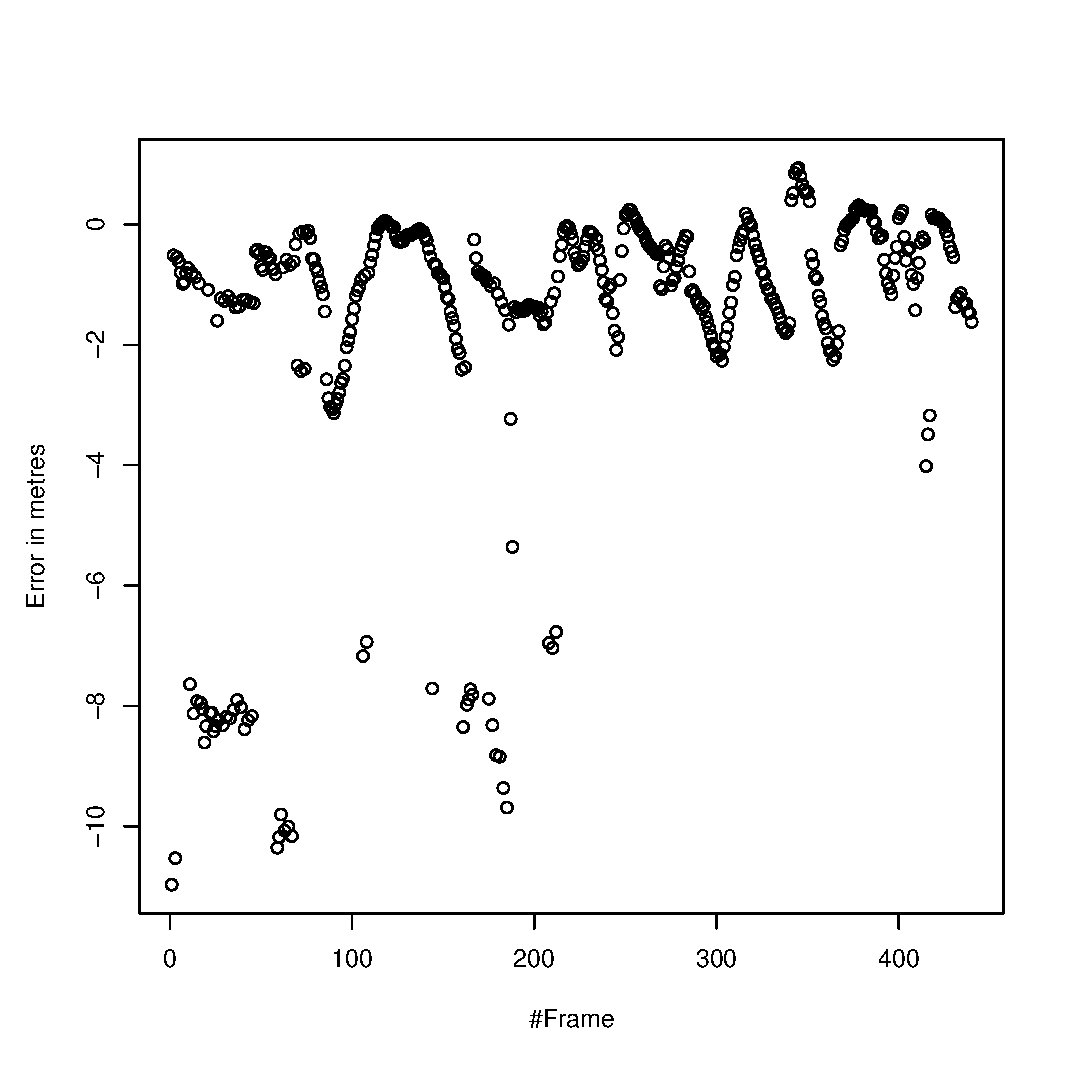
\includegraphics[width=\textwidth]{results/distance-error.eps}
  \end{minipage}
  \begin{minipage}[]{0.48\textwidth}
    \centering
    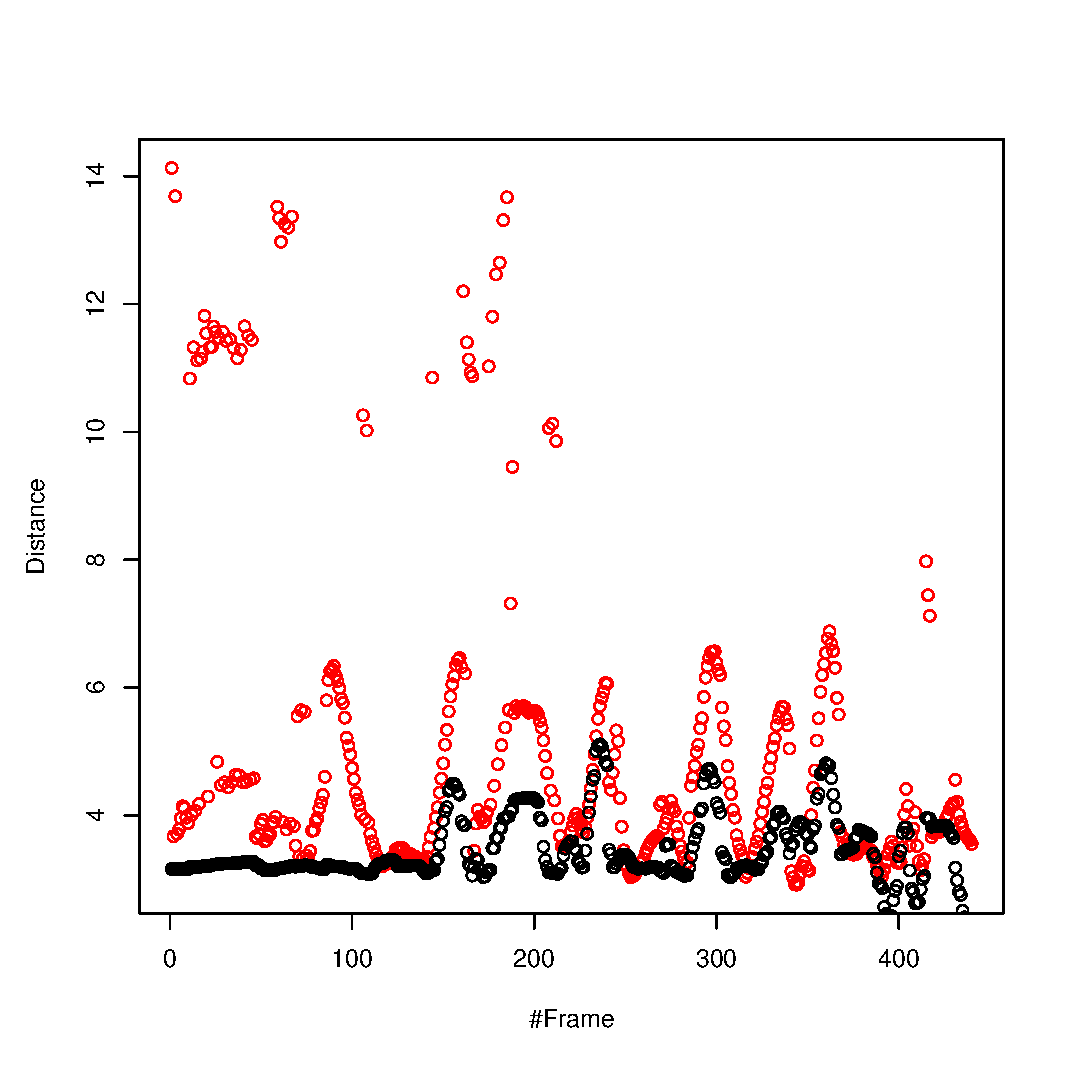
\includegraphics[width=\textwidth]{results/distance-comparason.eps}
  \end{minipage}
  \label{fig:err-dist}
    \caption{Comparison between true distance and predicted distance. The red points are the predictions, the right-most plot is the distance difference.}
\end{figure}

The distances of the tracked humans that we calculate for each frame are coherent
but not very accurate. There are two distinct ranges of error values.
The range with the lowest values corresponds to the actual calculation error, and the other one to the case when the chair or partial persons in the background are tracked.

As this chair is in general not close to the person wearing the distance marker,
the error is larger on those occasions.

\begin{figure}[H]
\centering
  \begin{minipage}[]{0.7\textwidth}
    \centering
    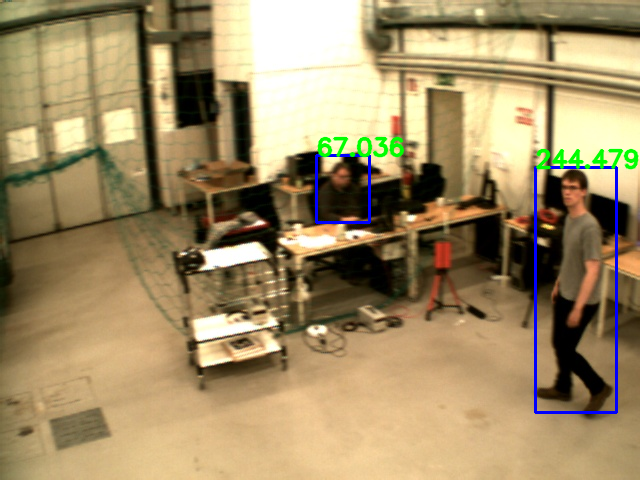
\includegraphics[width=\textwidth]{figures/example-frame.png}
  \end{minipage}
  \label{fig:fp-frame}
    \caption{Example of a video-frame with a false-positive.}
\end{figure}

The \emph{computation time} required for the detection step varies between
0.27 and 0.3 seconds and about 8\% of the frames contain false positive detections.

\subsection{LIDAR Tracking}

The training took 42 hours in total, the error from the loss function for different iterations can be shown in figure \ref{fig:loss}.

\begin{figure}[H]
  \begin{center}
    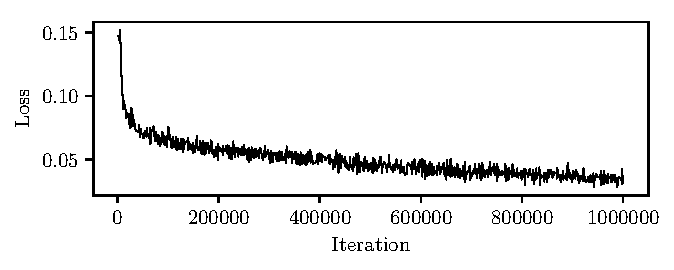
\includegraphics[width=\textwidth]{figures/loss-plot}
  \end{center}
  \caption{The loss for different number of iterations.}
  \label{fig:loss}
\end{figure}

The resulting performance can be shown in the videos \footnote{\url{https://youtu.be/9SNCCgjbLO8}}\footnote{\url{https://youtu.be/yVZY8ZJkqBk}}.

\section{Discussion}

\subsection{Camera Tracking}

A significant part of the dedicated project time was consumed by configuration problems.
This was due to several parameters. First, we had to achieve a good computation time,
so we wanted to use the GPU for the calculus, and we tried to do so in our personal machines.
The configuration work for that is quite heavy and touchy, such that we broke our
personal computer's systems a few times and had to reset everything and go back
from scratch. Each of us was also using a different operating system, such that
we couldn't always help each other and make our personal experience beneficial
to the group. We were also dealing with a project consisting in aggregating
multiple pieces of software, and they were all requiring different
configurations and relying on different dependencies.


This loss of time is the main reason why we didn't have time to implement YOLO
\footnote{https://pjreddie.com/darknet/yolo/},
which could have solved quite a few problems we encountered and looks very promising
in terms of performances.

The detection takes such a long time because the model we use is originally intended
to detect 20 different classes, and it computes the confidence score for all
those classes on all proposed bounding boxes. We then only consider the ones corresponding
to persons and continue the workflow, but that adds a certain overhead to the computation
of the detection. This can be further improved but we didn't have time to do so,
thus we don't know to what extent this detection time can be reduced. This might
also be solved using YOLO.

The distance estimation is not very accurate because the bounding boxes don't
match the human shape very accurately, i.e. sometimes it will cut a bit of its head
or feet and sometimes it will encompass the whole human even with some margins.
As we are basing our estimation of the distance on the average human height and
the height of the bounding box yields varying results for the same distance. The top-down angle of the camera and the estimation of the height of the person (which is an estimation,
thus not their exact height) can also have an impact on this shift.

The detector is too good at detecting partial humans, which is a good thing in a
general application but is a problem for us as we are calculating the distance of
the tracked targets based on the average human height and the height of the bounding
box of the target. That's why when we detect the chest of a human sat behind a table,
we place it further than its actual location because the bounding box is half
the size it should be if the person was standing. This problem might be solved using YOLO.
% TODO: Why is this sentence starting with a lower-case t? Is it a cut-off sentence or just a small error?

\subsection{LIDAR Tracking}

% Explain the differences
The main differences between the implementations are performance and training time.
In both cases the system performs worse, it takes longer to train and when trained it performs worse.

% Why does training take a longer time?
One difference is that the original system in Torch uses an explicit training loop, where a sequence of images is preprocessed, fed into the network, backpropagation is calculated and then finally the weights are updated.
The new system, written in TensorFlow, uses an implicit training loop which is not entirely understood by the project members.
The training loop takes an error function as input, a set of data divided into batches and a number of iterations to perform.
In order to mimic that the weights are updated for every sequence of images the new system uses the same number of images per batch as the sequence in the original training process.
It also uses a batch size equal to one, in order to update the weights after every such sequence of images.
This could explain partly why the training takes longer.

% Discuss how the preprocessing could be done in a more efficient manner
The preprocessing is not implemented in an ideal manner.
In the original Lua implementation the preprocessing is done on the fly, meaning that whenever an image was needed it was calculated from the raw LIDAR data.
However, in TensorFlow it is easier to supply all data in the beginning as NumPy arrays.
There are two alternatives which could be more memory efficient.
First, the data could be preprocessed offline on a machine with more working memory and saved to some file format native to either NumPy or TensorFlow.
This could shrink the memory needed by quite a bit, as there does not need to be two representations of the data set in memory at the same time.
Second, the preprocessing could be done directly in TensorFlow by using TensorFlow operations on the data rather than NumPy operations.
This could allow it to be done on the fly, as in the original implementation.

% Point out the possibility of unknown errors
Lastly, it is also possible that the difference is performance is caused by some unknown error.
For example, the error which resulted in only 721 time-steps being included in the training data was caused by an error with indexing.
In this case the underlying problem was that Lua and Python uses different indexing systems, Lua starts at 1 while Python starts 0 when indexing vectors and matrices.
The error was small, but had large consequences and did not cause any warning or error messages.
Furthermore, the error occurred even though the authors were aware of the difference between the languages.
There are probably more or less critical hidden problems, however not necessarily related to indexing.

\section{Conclusion}

Looking at the two approaches examined in this report we can see that both have some merit but also some drawbacks.

The camera tracking resulted in very roughs distance estimations and SORT required to much computational time to be usable in a real-time system. Going forward with a camera-based approach we would recommend switching to YOLO for detections but the pinhole model seemed promising for distance estimations.

When looking at the LIDAR-based approach we find it promising, even though the new implementation has its flaws.
There are advantages to LIDAR-based tracking, a LIDAR sweep contains is considerably smaller than an image from a camera but still contain more than enough information to successfully track objects.
This makes real-time tracking more easily achievable at the cost of having less information about the world.

\printbibliography

\end{document}
